% !TEX root = ../../thesis.tex
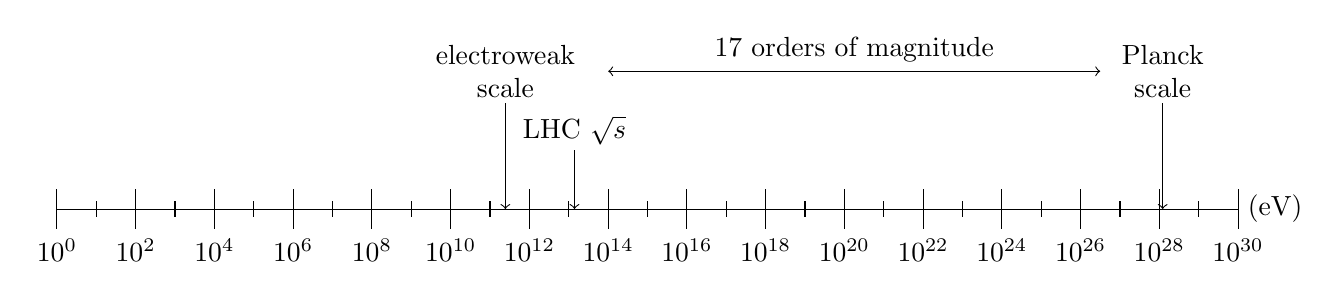
\begin{tikzpicture}
  % Axis
  \draw (0,0) -- (15,0) node[right] {(eV)};
  \draw (0,-0.25) -- (0,0.25);
  \node[below] at (0,-0.25) {$10^0$};

  \foreach \i in {1,...,15}
  {
    % Ticks
    \pgfmathsetmacro{\y}{\i-0.5}
    \draw (\i,-0.25) -- (\i,0.25);
    \draw (\y,-0.1) -- (\y,0.1);

    % Numerical labels
    \pgfmathtruncatemacro{\x}{\i*2}
    \node[below] at (\i,-0.25) {$10^{\x}$};
  }

  % Labels
  \draw[->] (5.695,1.75) node[fill=white,inner sep=2pt,align=center] {electroweak\\scale} -- (5.695,0);
  \draw[->] (6.573,1) node[fill=white,inner sep=2pt] {LHC $\sqrt{s}$} -- (6.573,0);
  \draw[->] (14.043,1.75) node[fill=white,inner sep=2pt,align=center] {Planck\\scale} -- (14.043,0);
  \draw[<->] (7,1.75) -- (13.25,1.75) node[pos=0.5,above] {17 orders of magnitude};
\end{tikzpicture}
